\documentclass[11pt]{article}
\usepackage[margin=1in]{geometry}
\usepackage{graphicx}
\usepackage{amsmath}
\usepackage{booktabs}
\usepackage{hyperref}
\usepackage{siunitx}

\title{ADS-B-Guided Weak-Target Radar Tracking Under Low SNR and Clutter}
\author{Your Name \\ Your Institution}
\date{\today}
\begin{document}
\maketitle
\begin{abstract}
Radar detection forces a threshold tradeoff: a high threshold suppresses clutter but loses weak targets, while a low threshold recovers weak targets and floods the tracker with clutter-induced false tracks. We build an ADS-B-grounded evaluation framework in which real fixed-wing general-aviation trajectories from OpenSky are cleaned, relocated into a synthetic radar's coordinate frame, and converted into noisy, cluttered radar \emph{point detections}. On this framework we compare a ladder of methods: threshold-only detection, a constant-velocity Kalman tracker, hand-designed physics scoring, empirical ADS-B motion priors, learned sequence autoencoders, a variational autoencoder, and a diffusion denoiser. Our selected method is a deterministic sequence autoencoder scored by reconstruction error over origin- and heading-normalized trajectory windows, with an error-to-score mapping calibrated on high-purity \emph{noisy} tracks rather than clean truth. This noise-matched calibration is essential: without it, true-track retention collapses. Over four days and thresholds $-5$ to $6$\,dB, the Kalman baseline yields \num{323808} true and \num{815} false tracks; our method retains \SI{97.3}{\percent} of true tracks while removing \SI{99.39}{\percent} of false tracks, keeping only 5 of \num{815}. We emphasise scope: this is a point-detection simulation, not a raw RF or range-Doppler intensity simulation.
\end{abstract}
\section{Introduction}
A radar detector's threshold sets an unavoidable operating point. Raising it removes clutter at the cost of weak targets; lowering it recovers weak targets but presents the tracker with many clutter detections, which associate into false tracks. Single-frame reasoning cannot separate a weak target from a clutter point. Trajectory-level reasoning can, because aircraft motion has temporal structure that clutter chains do not reproduce. This paper asks how much of the false-track burden trajectory-shape reasoning can remove, how it must be calibrated, and whether the result survives across days.
\begin{figure}[htbp]
  \centering
  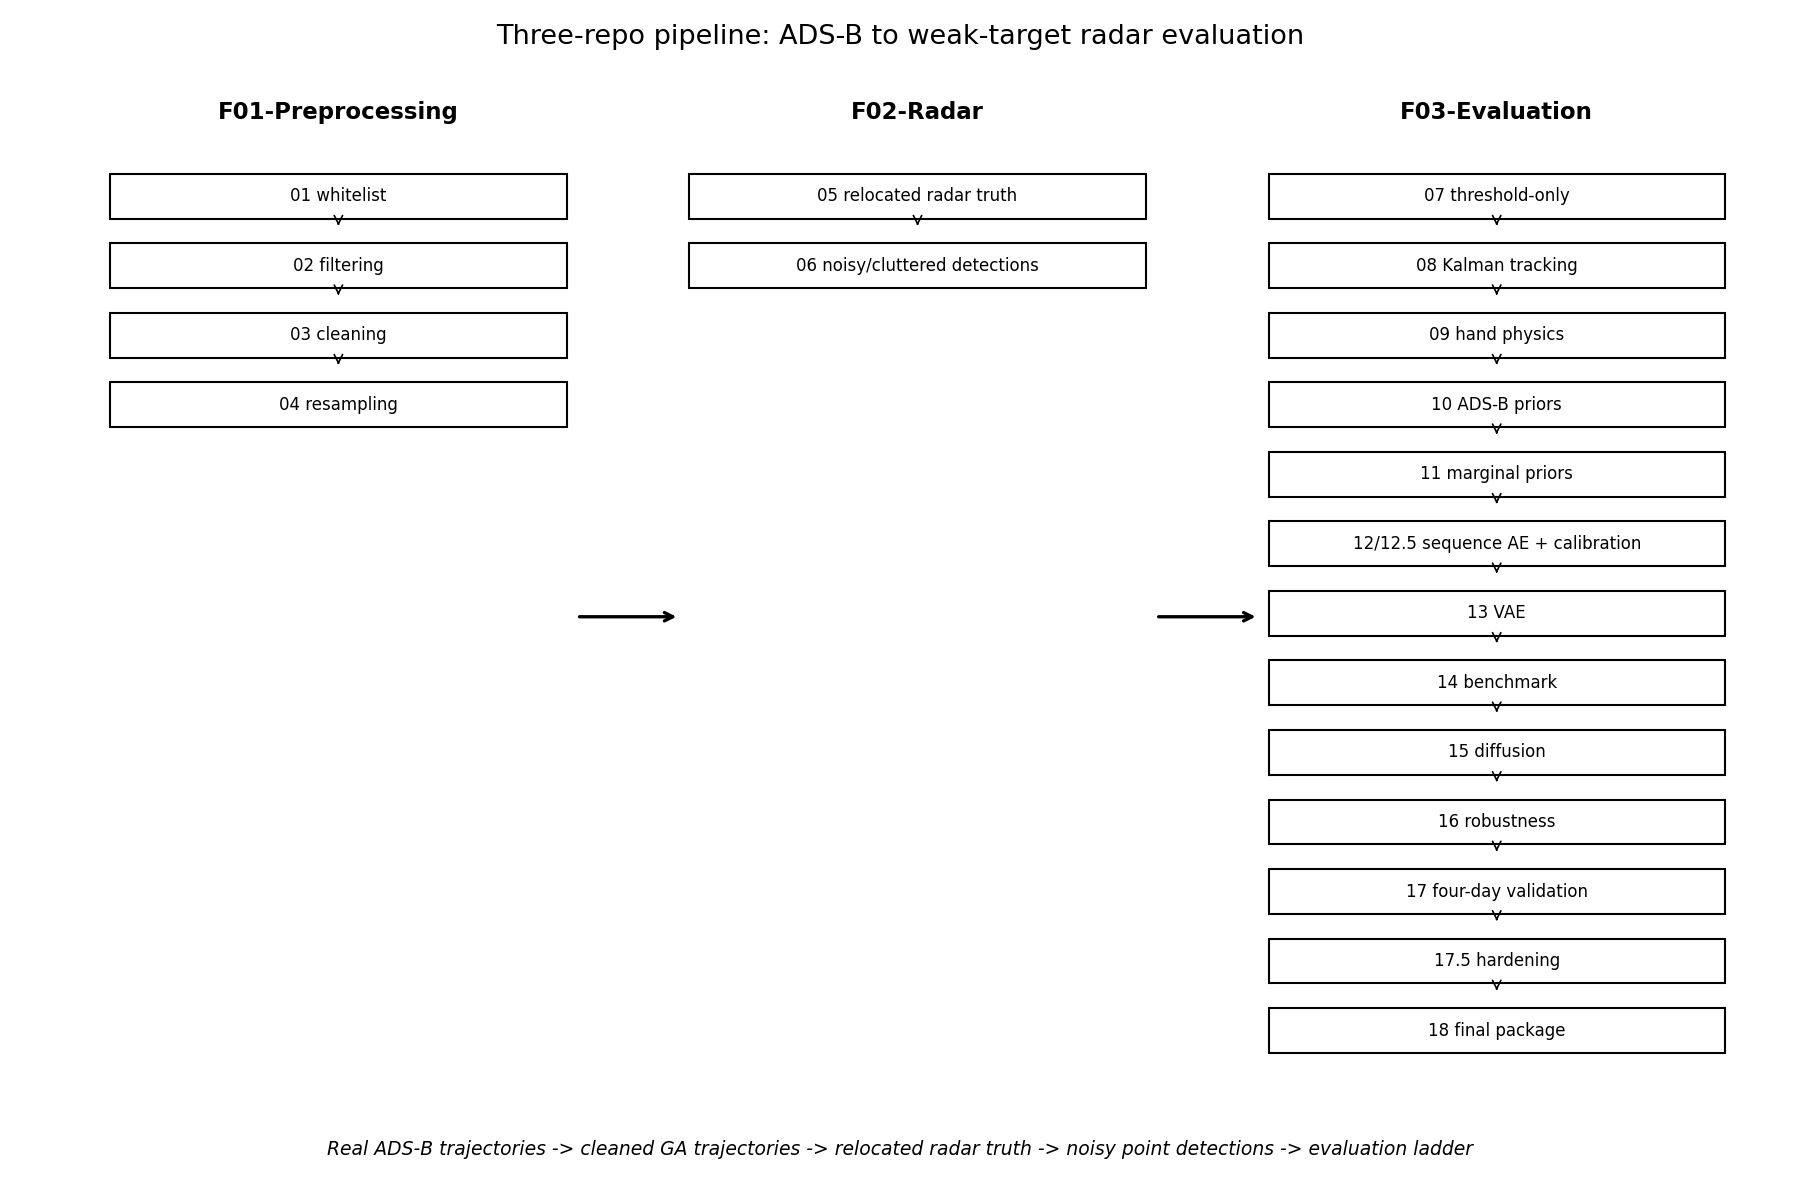
\includegraphics[width=0.92\linewidth]{figures/01_pipeline_diagram.png}
  \caption{Three-repo pipeline from real ADS-B trajectories to weak-target radar evaluation.}
  \label{fig:pipeline}
\end{figure}

\section{Related work}
Recursive state estimation for tracking dates to the Kalman filter~\cite{kalman1960}. Track-before-detect approaches integrate energy across frames before thresholding to recover weak targets~\cite{tbd}. Our detections derive from the OpenSky network~\cite{opensky}, a widely used source of real ADS-B trajectories, and trajectory-prediction work has established that ADS-B motion is highly structured~\cite{adsbpred}. Our scoring uses reconstruction error from an autoencoder as an anomaly signal~\cite{aeanomaly}, and we additionally evaluate a variational autoencoder~\cite{vae} and a denoising diffusion model~\cite{ddpm}. Our contribution is not any one of these components but their integration into an ADS-B-grounded weak-target evaluation framework, together with the noise-matched calibration that makes the learned score usable on noisy tracks.
\section{Data and simulation pipeline}
Real OpenSky ADS-B tracks are whitelisted to fixed-wing general aviation, filtered, cleaned, and resampled onto a uniform \SI{10}{\second} grid. Trajectories are then \emph{relocated}: each trajectory's start anchor is placed in a \SIrange{10}{80}{\km} annulus around a synthetic radar using a per-trajectory SHA-256-derived seed, preserving the real motion shape while bringing the engagement geometry under experimental control.
\begin{figure}[htbp]
  \centering
  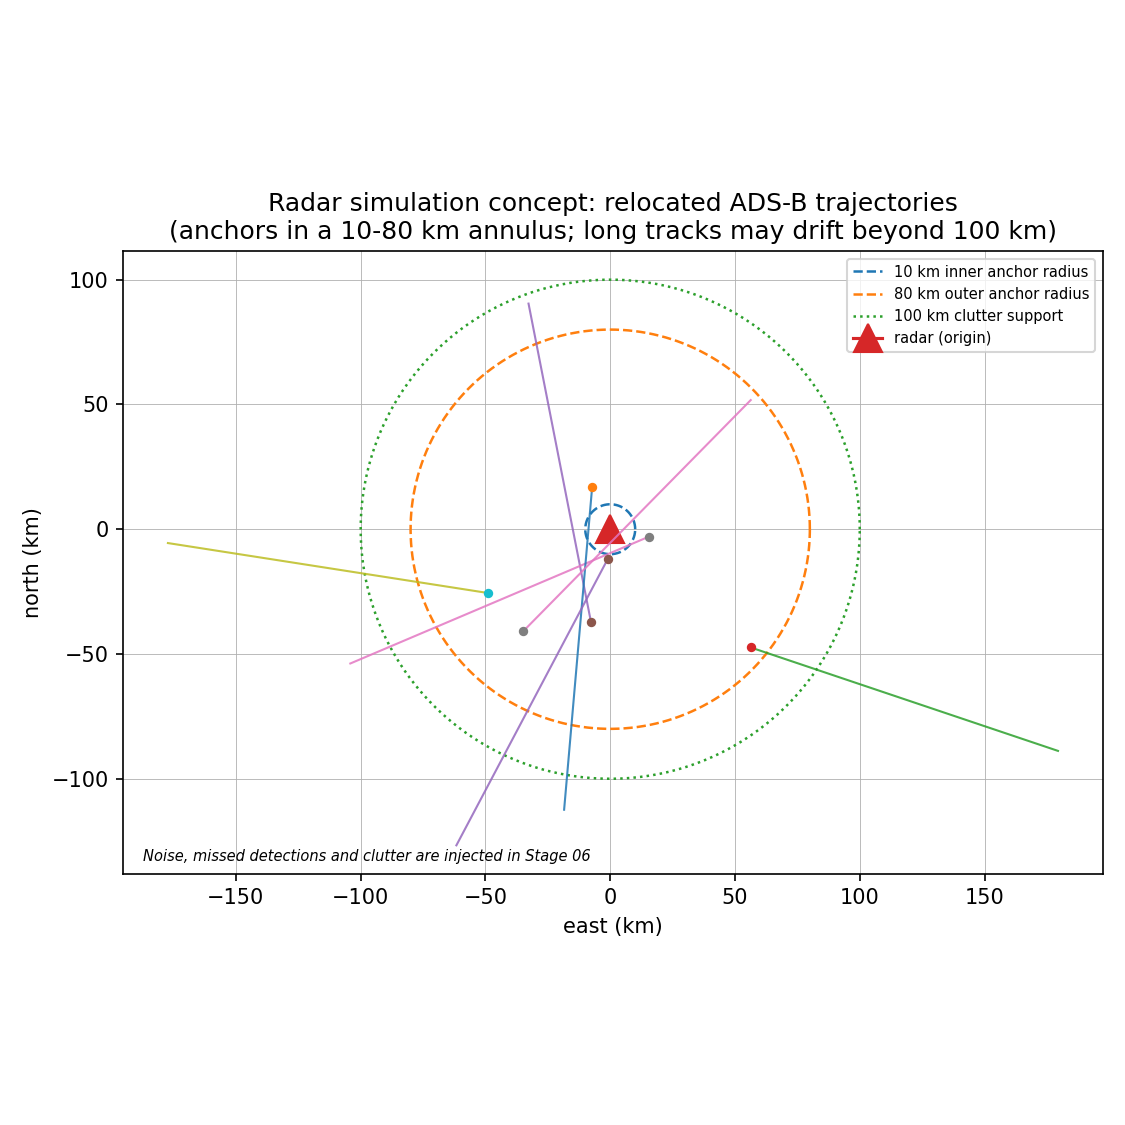
\includegraphics[width=0.92\linewidth]{figures/02_radar_simulation_concept.png}
  \caption{Radar simulation concept: relocated ADS-B trajectories anchored in a 10--80\,km annulus around the radar.}
  \label{fig:concept}
\end{figure}

\section{Radar point-detection simulation}
The radar model produces \emph{point detections} per scan: an $R^{-4}$ SNR decay, a logistic probability of detection, per-component measurement noise on range, azimuth, elevation and radial velocity, and Poisson clutter. \textbf{There is no raw RF/IQ and no gridded range-Doppler intensity simulation.} Accordingly, the range-Doppler figure below is a scatter plot of point detections, not a radar intensity map.
\begin{figure}[htbp]
  \centering
  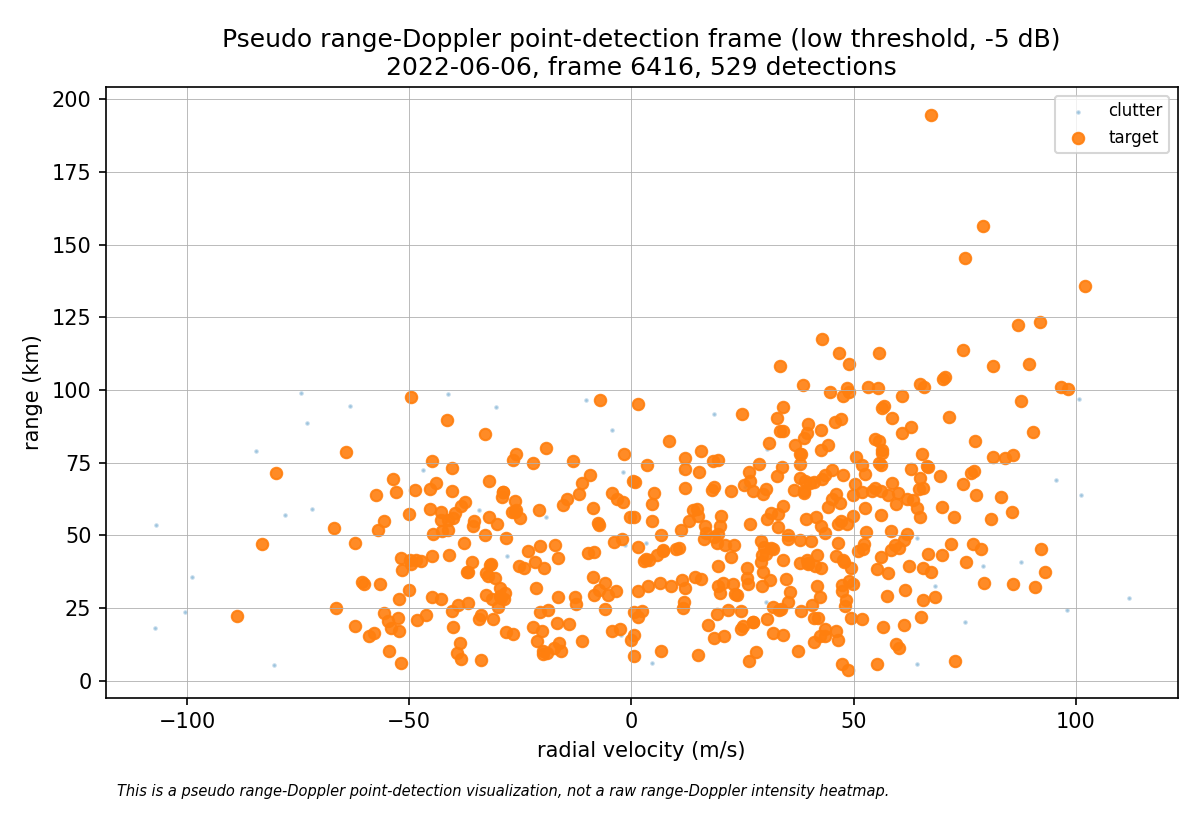
\includegraphics[width=0.92\linewidth]{figures/03_pseudo_range_doppler_frame_low_threshold.png}
  \caption{Pseudo range-Doppler point-detection frame at the low threshold ($-5$\,dB). This is a point-detection pseudo range-Doppler visualization, not a raw radar intensity map.}
  \label{fig:rdlow}
\end{figure}

\begin{figure}[htbp]
  \centering
  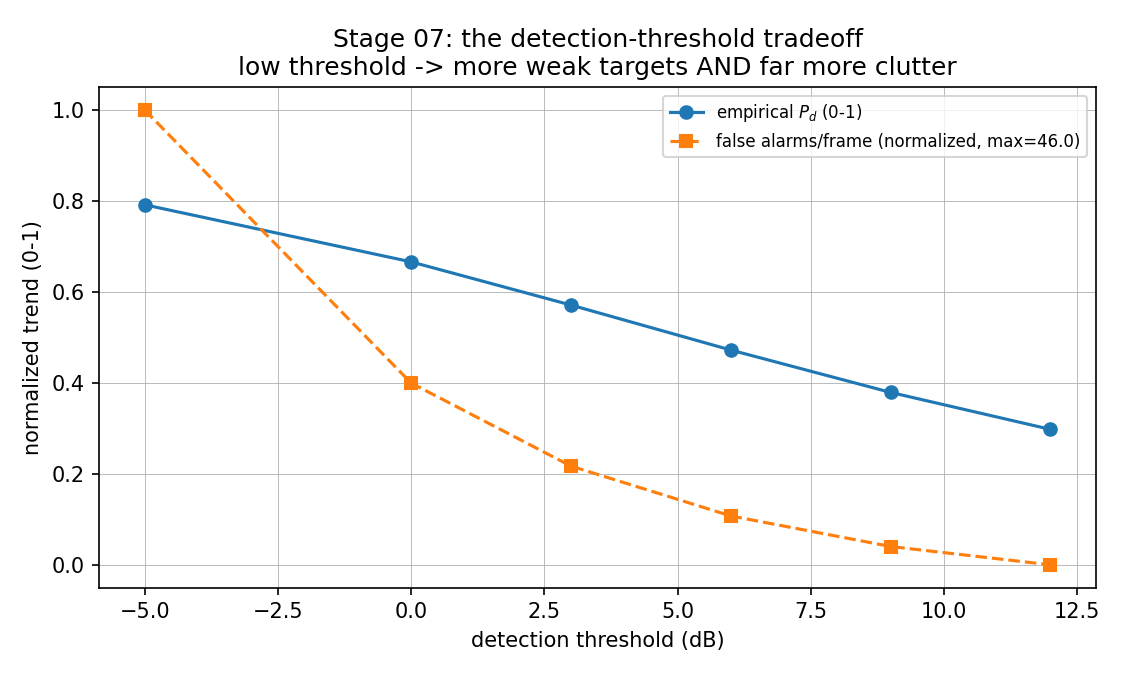
\includegraphics[width=0.92\linewidth]{figures/07_threshold_tradeoff_stage07.png}
  \caption{The detection-threshold tradeoff: lowering the threshold recovers weak targets but multiplies clutter.}
  \label{fig:tradeoff}
\end{figure}

\section{Method ladder}
We evaluate, in order: threshold-only detection (frame level); a constant-velocity Kalman tracker with greedy gated nearest-neighbour association, which defines the true/false-track denominator; hand-designed physics scoring; empirical marginal ADS-B motion priors; learned sequence autoencoders; a VAE trajectory prior; and a diffusion denoiser. The tracker never sees truth labels; labels enter only in evaluation.
\begin{figure}[htbp]
  \centering
  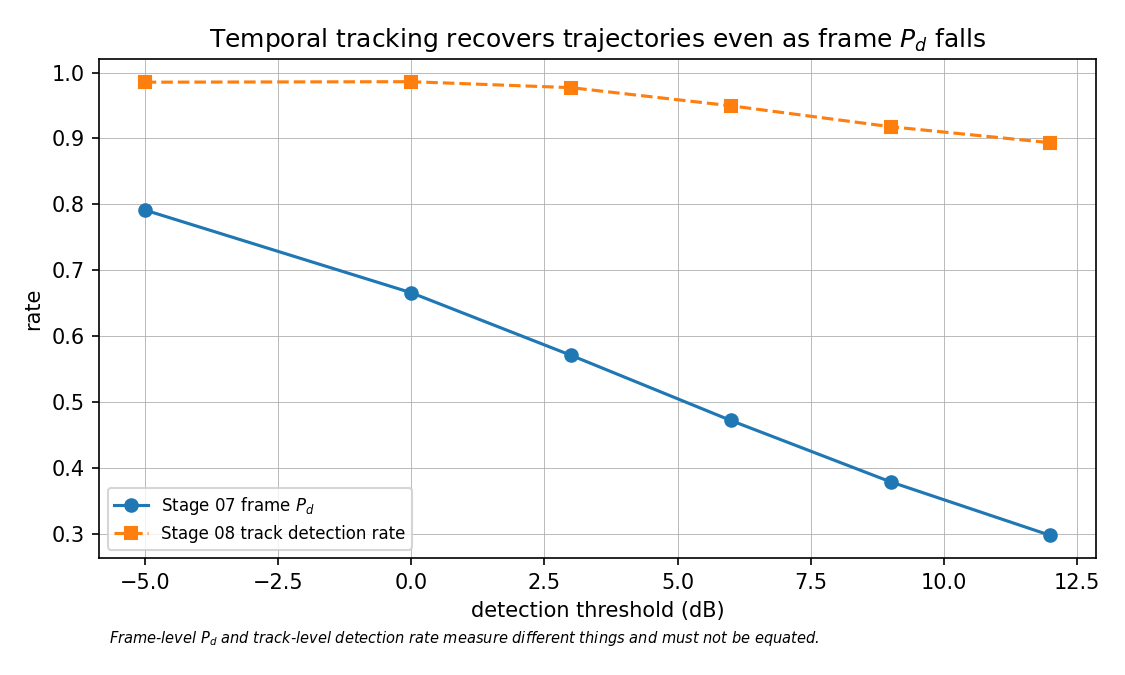
\includegraphics[width=0.92\linewidth]{figures/08_kalman_tracking_effect_stage08.png}
  \caption{Temporal tracking recovers trajectories even as frame-level $P_d$ falls.}
  \label{fig:tracking}
\end{figure}

\begin{figure}[htbp]
  \centering
  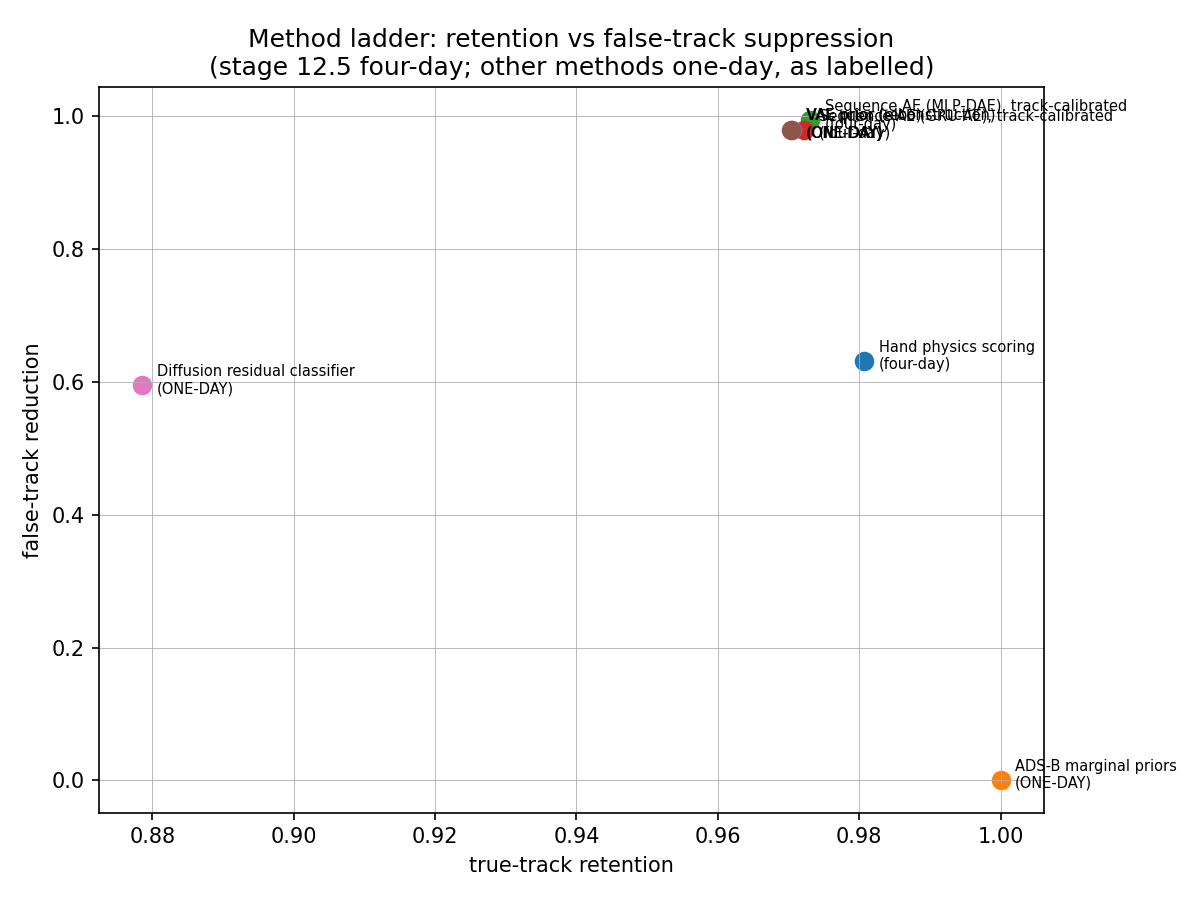
\includegraphics[width=0.92\linewidth]{figures/11_method_ladder_comparison.png}
  \caption{Method ladder: true-track retention against false-track reduction.}
  \label{fig:ladder}
\end{figure}

\section{Sequence-prior calibration}
Trajectory windows are origin-shifted and heading-rotated so the model learns motion \emph{shape}. A denoising autoencoder is trained on clean truth windows, and a track is scored by the median per-window reconstruction error of its Kalman posterior. Mapping that error to a score using \emph{clean-truth} quantiles is a domain shift: genuine tracks are posteriors over noisy measurements and reconstruct worse than clean truth, so they collapse toward score zero and true-track retention falls to roughly $0.08$. Re-anchoring the $p_{50}/p_{99}$ band on high-purity \emph{noisy} tracks restores retention to roughly $0.96$ with essentially no loss of false-track suppression. We call this \emph{noise-matched calibration}; it is the decisive step.
\begin{figure}[htbp]
  \centering
  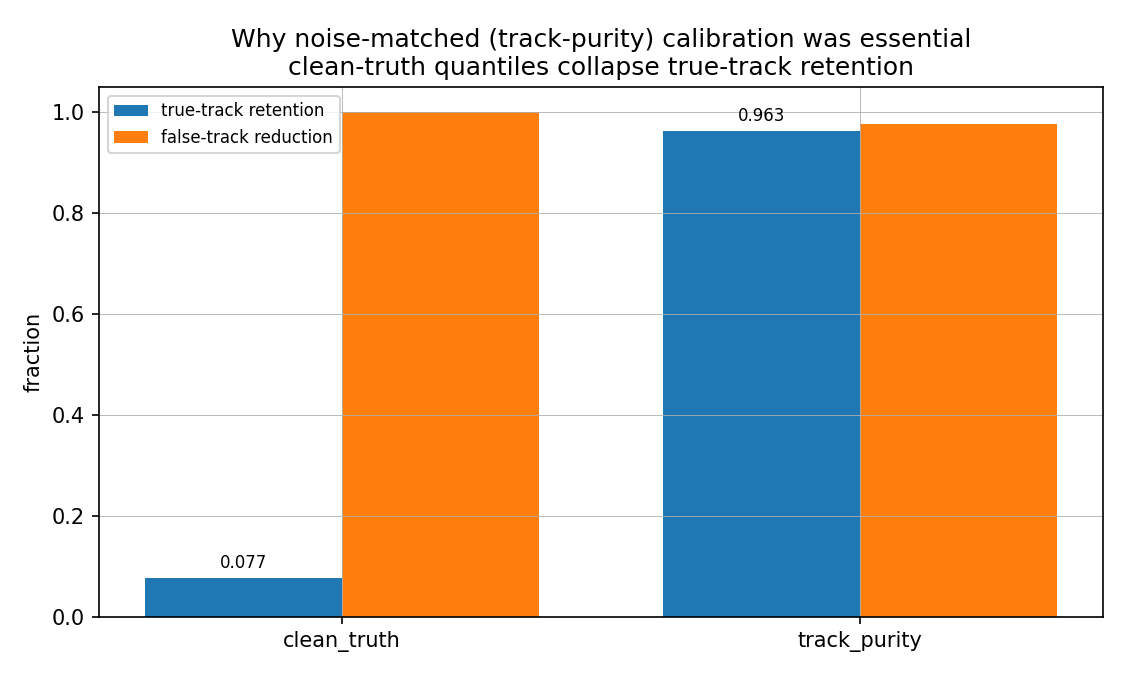
\includegraphics[width=0.92\linewidth]{figures/10_stage12_calibration_effect.png}
  \caption{Noise-matched (track-purity) calibration is what makes the learned score usable.}
  \label{fig:calib}
\end{figure}

\section{Results}
Across four days at $-5/0/3/6$\,dB the Kalman baseline yields \num{323808} true and \num{815} false confirmed tracks. The selected method retains \SI{97.3}{\percent} of true tracks and removes \SI{99.39}{\percent} of false tracks, keeping 5 of \num{815}. Results are stable across days (Fig.~\ref{fig:fourdayret}, Fig.~\ref{fig:beforeafter}).
\begin{figure}[htbp]
  \centering
  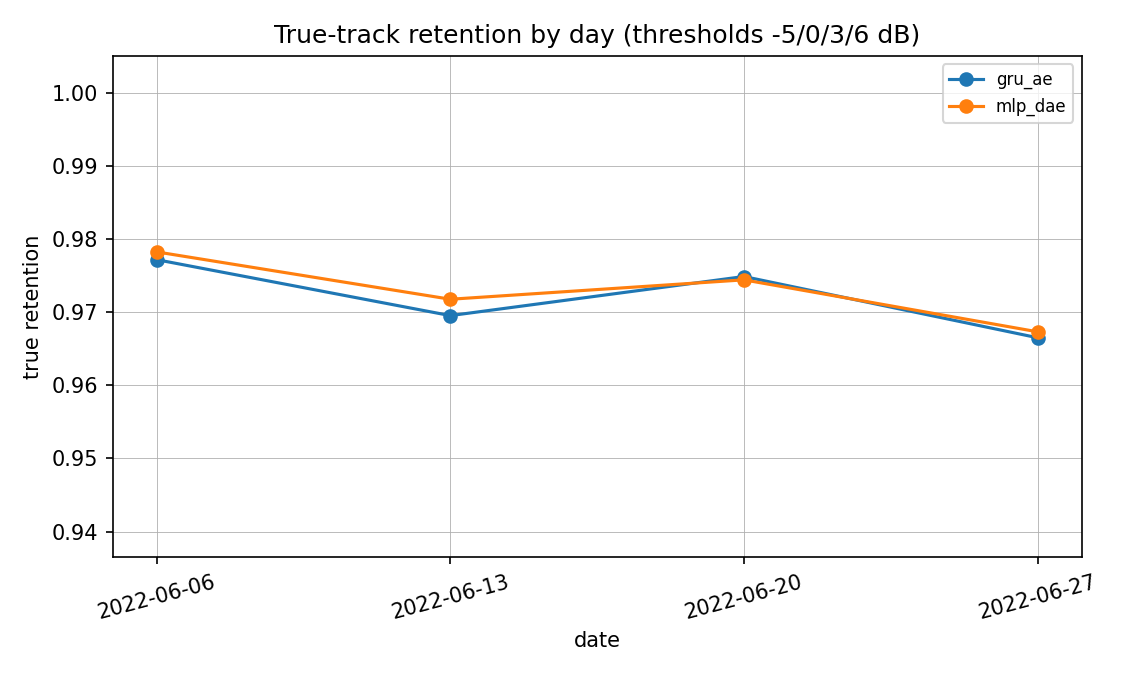
\includegraphics[width=0.92\linewidth]{figures/12_four_day_validation_retention.png}
  \caption{True-track retention across all four days.}
  \label{fig:fourdayret}
\end{figure}

\begin{figure}[htbp]
  \centering
  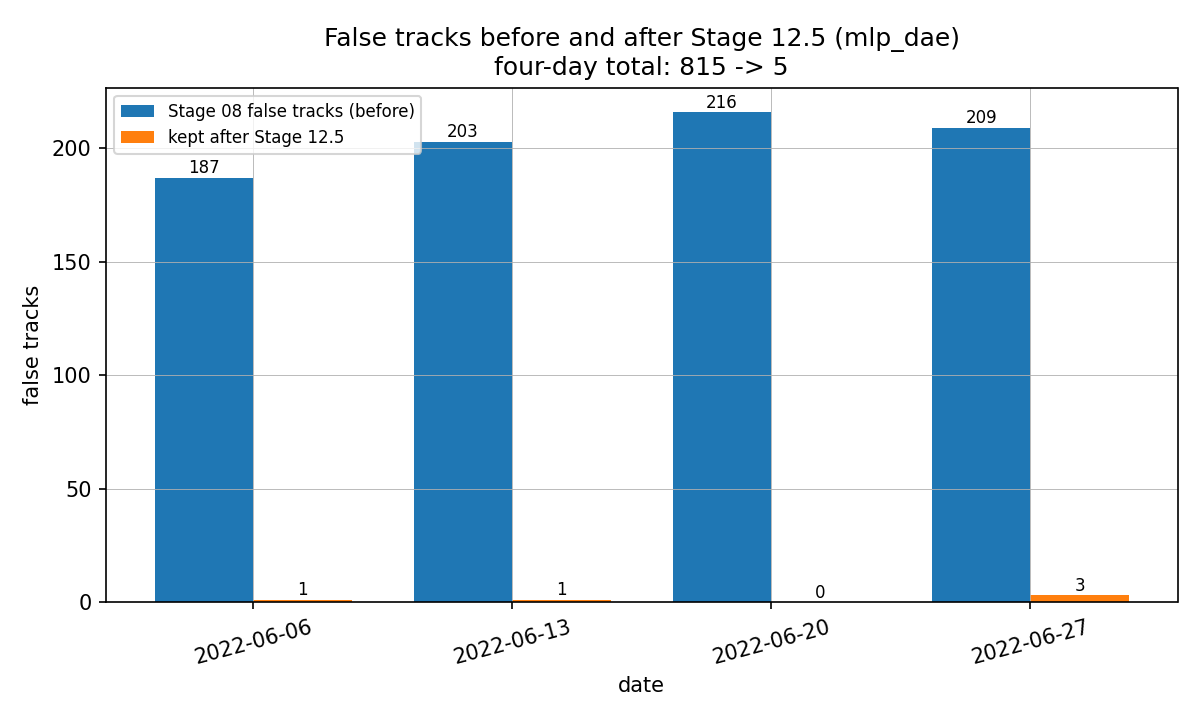
\includegraphics[width=0.92\linewidth]{figures/14_false_tracks_before_after_stage12.png}
  \caption{False tracks before and after Stage~12.5.}
  \label{fig:beforeafter}
\end{figure}

\begin{table}[htbp]
  \centering
  \small
  \begin{tabular}{lllll}
    \hline
    method & stage & true\_retention & false\_reduction & scope \\
    \hline
    Kalman only & 08 & 1.0000 & 0.0000 & four-day (-5..6 dB) \\
    Hand physics scoring & 09 & 0.9807 & 0.6315 & four-day (-5..6 dB) \\
    ADS-B marginal priors & 11 & 1.0000 & 0.0012 & ONE-DAY (2022-06-06) \\
    Sequence AE (MLP-DAE), track-calibrated & 12.5 & 0.9731 & 0.9939 & four-day (-5..6 dB) \\
    Sequence AE (GRU-AE), track-calibrated & 12.5 & 0.9722 & 0.9791 & four-day (-5..6 dB) \\
    VAE prior (elbo) & 13 & 0.9705 & 0.9798 & ONE-DAY (2022-06-06) \\
    VAE prior (reconstruction) & 13 & 0.9704 & 0.9798 & ONE-DAY (2022-06-06) \\
    Diffusion residual classifier & 15 & 0.8786 & 0.5948 & ONE-DAY (2022-06-06) \\
    \hline
  \end{tabular}
  \caption{Method comparison. Stage~12.5 rows are four-day; rows marked ONE-DAY were evaluated on a single day.}
  \label{tab:methods}
\end{table}

\section{Ablations}
Calibration dominates: clean-truth versus track-purity calibration is the difference between an unusable and a usable filter. Among model families, the MLP autoencoder is best overall and the GRU is a close second, while the TCN retains fewer true tracks. The VAE does not beat the deterministic autoencoder, and the diffusion residual is clearly worse as a classifier, although diffusion does regularize tracks and modestly improves gap filling. Hand-designed physics scoring remains a strong interpretable fallback.
A denominator caveat applies at high thresholds: sequence methods only score tracks long enough to window, and at $9$/$12$\,dB essentially no false track is that long, so false-track reduction is \emph{undefined} rather than zero or one (Fig.~\ref{fig:window}).
\begin{figure}[htbp]
  \centering
  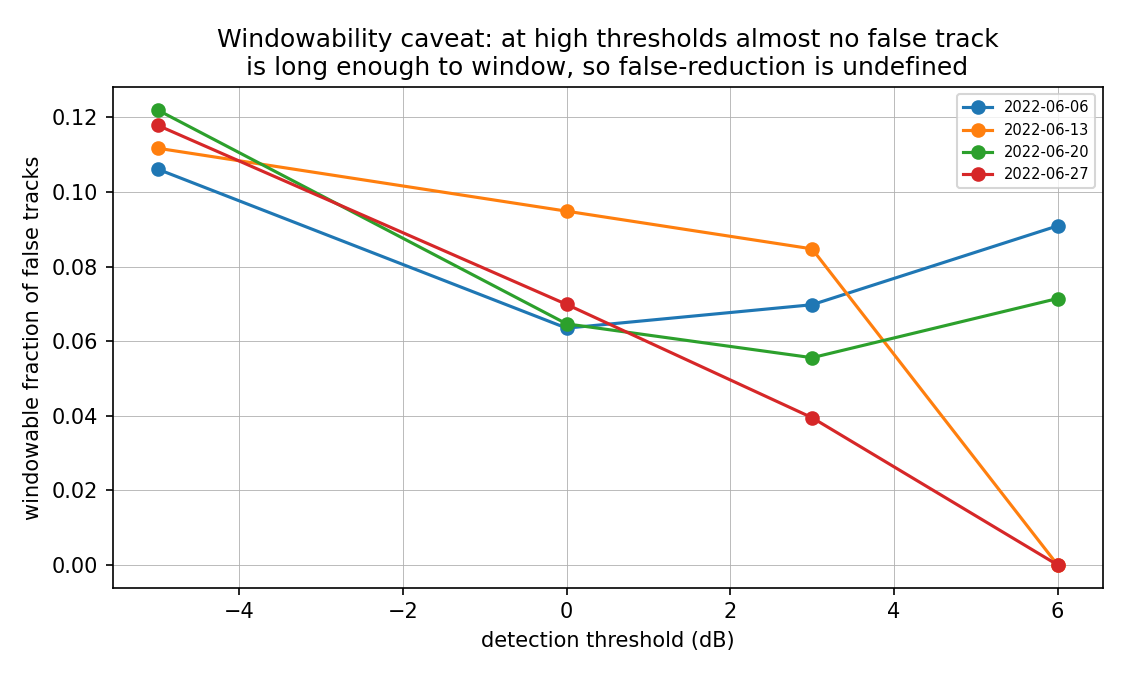
\includegraphics[width=0.92\linewidth]{figures/17_windowability_caveat.png}
  \caption{Windowability caveat: at high thresholds almost no false track is long enough to window, so false-track reduction is undefined.}
  \label{fig:window}
\end{figure}

\section{Limitations}
\begin{itemize}
  \item Point-detection radar simulation, not raw RF/IQ
  \item Pseudo range-Doppler figures are point-detection scatter plots
  \item Synthetic relocation of trajectories near the radar
  \item OpenSky ADS-B-derived fixed-wing GA focus
  \item High-threshold windowability caveat (9/12 dB)
  \item Track-purity calibration uses truth labels to SELECT calibration tracks
  \item Learned-method evidence is on simulated detections, not real radar returns
  \item Diffusion and VAE were not tuned exhaustively
  \item Runtime / deployment not optimized
\end{itemize}
\section{Conclusion}
The novelty is not in Kalman filtering, autoencoders, or radar thresholding individually. The contribution is an ADS-B-grounded weak-target radar evaluation framework and a noise-matched learned trajectory-shape scoring method that suppresses low-threshold clutter-induced false tracks while retaining true aircraft tracks, demonstrated across four days.
\bibliographystyle{plain}
\bibliography{references}
\end{document}